\documentclass[11pt,a4paper]{article}

% Image mode: pdf.
% Image paths stay relative. In PDF mode, place same-basename PDF conversions
% of the chapter SVG files in the assets/ directory beside this source.

\usepackage{iftex}
\ifPDFTeX
  \PackageError{handout}{This template requires XeTeX or Tectonic}{Compile with xelatex or tectonic.}
\fi

\usepackage[a4paper,top=18mm,bottom=20mm,left=20mm,right=20mm,headsep=6mm]{geometry}
\usepackage{fontspec}
\usepackage{xeCJK}
\usepackage{amsmath}
\usepackage{unicode-math}

% Font settings are intentionally visible in the generated .tex file.
% These defaults target the macOS machine used for the released PDF.
% Change the family names when compiling on another system.
\setmainfont{Songti TC}
\setsansfont{Heiti TC}
\setmonofont{Menlo}
\setCJKmainfont{Songti TC}
\setCJKsansfont{Heiti TC}
\setCJKmonofont{Heiti TC}
\setmathfont{STIX Two Math}
\XeTeXlinebreaklocale "zh"
\XeTeXlinebreakskip=0pt plus 1pt

\usepackage{xcolor}
\definecolor{HandoutBlue}{HTML}{215A91}
\definecolor{HandoutBlueLight}{HTML}{EEF5FC}
\definecolor{HandoutGreen}{HTML}{39715A}
\definecolor{HandoutGreenLight}{HTML}{EFF8F3}
\definecolor{HandoutGold}{HTML}{8A641C}
\definecolor{HandoutGoldLight}{HTML}{FFF8E8}
\definecolor{HandoutInk}{HTML}{253142}
\definecolor{HandoutMuted}{HTML}{667085}

\usepackage{graphicx}
\makeatletter
% Pandoc 3 emits an accessibility `alt` key for raster/PDF images. Older
% graphicx releases do not know that key, so accept it without changing layout.
\@ifundefined{KV@Gin@alt}{\define@key{Gin}{alt}{}}{}
\newsavebox\pandoc@box
\newcommand*\pandocbounded[1]{%
  \sbox\pandoc@box{#1}%
  \Gscale@div\@tempa{\textheight}{\dimexpr\ht\pandoc@box+\dp\pandoc@box\relax}%
  \Gscale@div\@tempb{\linewidth}{\wd\pandoc@box}%
  \ifdim\@tempb\p@<\@tempa\p@\let\@tempa\@tempb\fi
  \ifdim\@tempa\p@<\p@\scalebox{\@tempa}{\usebox\pandoc@box}%
  \else\usebox{\pandoc@box}%
  \fi
}
\makeatother
\usepackage{float}
\floatplacement{figure}{H}
% Pandoc uses LTcaptype=none for uncaptioned longtables. The caption package
% expects that name to exist as a counter even though it is never displayed.
\newcounter{none}
\usepackage{caption}
\captionsetup[figure]{labelformat=empty,labelsep=none,font=small}

\usepackage{booktabs,longtable,array,calc}
\usepackage{etoolbox}
\makeatletter
\patchcmd\longtable{\par}{\if@noskipsec\mbox{}\fi\par}{}{}
\makeatother

\usepackage[most]{tcolorbox}
\tcbuselibrary{breakable,skins}
\newtcolorbox{HandoutLearningMap}{
  enhanced,breakable,colback=HandoutBlueLight,colframe=HandoutBlue,
  boxrule=0.8pt,arc=1.5mm,left=3mm,right=3mm,top=2mm,bottom=2mm,
  before skip=8pt,after skip=10pt
}
\newtcolorbox{HandoutWorkedExample}{
  enhanced,breakable,colback=HandoutGreenLight,colframe=HandoutGreen,
  boxrule=0.65pt,arc=1.5mm,left=3mm,right=3mm,top=2mm,bottom=2mm,
  before skip=8pt,after skip=10pt
}
\newtcolorbox{HandoutSelfCheck}{
  enhanced,breakable,colback=HandoutGoldLight,colframe=HandoutGold,
  boxrule=0.65pt,arc=1.5mm,left=3mm,right=3mm,top=2mm,bottom=2mm,
  before skip=8pt,after skip=10pt
}

\usepackage{titlesec}
\titleformat{\section}{\sffamily\bfseries\Large\color{HandoutBlue}}{}{0pt}{}
\titleformat{\subsection}{\sffamily\bfseries\large\color{HandoutInk}}{}{0pt}{}
\titleformat{\subsubsection}{\sffamily\bfseries\normalsize\color{HandoutInk}}{}{0pt}{}
\titlespacing*{\section}{0pt}{1.4em}{0.55em}
\titlespacing*{\subsection}{0pt}{1.15em}{0.45em}
\titlespacing*{\subsubsection}{0pt}{0.9em}{0.35em}
\setcounter{secnumdepth}{-\maxdimen}

\usepackage{hyperref}
\usepackage{bookmark}
\IfFileExists{xurl.sty}{\usepackage{xurl}}{}
\urlstyle{same}
\hypersetup{
  colorlinks=true,
  linkcolor=HandoutBlue,
  urlcolor=HandoutBlue,
  citecolor=HandoutBlue,
  pdftitle={數1-1 數與式},
  pdfsubject={數學},
  pdfcreator={Pandoc with the HighSchooContent LaTeX template}
}

\setlength{\parindent}{0pt}
\setlength{\parskip}{0.55em plus 0.15em minus 0.1em}
\setlength{\emergencystretch}{3em}
\setlength{\LTpre}{0.5em}
\setlength{\LTpost}{0.5em}
\renewcommand{\arraystretch}{1.18}
\providecommand{\tightlist}{%
  \setlength{\itemsep}{0pt}\setlength{\parskip}{0pt}}
\pagestyle{plain}


\begin{document}

\begin{tcolorbox}[
  enhanced,colback=white,colframe=HandoutBlue,boxrule=1.1pt,arc=2mm,
  borderline west={3pt}{0pt}{HandoutBlue},left=5mm,right=4mm,top=4mm,bottom=4mm
]
{\sffamily\small\bfseries\color{HandoutBlue}學生講義}\par
{\sffamily\bfseries\LARGE\color{HandoutInk}數1-1 數與式}\par
\vspace{0.35em}{\large 用數線整理實數，以代數結構控制式的運算與最佳化}\par
\vspace{0.45em}{\small\color{HandoutMuted}%
科目：數學
\quad 課程：普通高中數學 第一冊
\quad 版本：學生版｜核心＋理解
\quad 校訂：2026-08-29
}\par
\vspace{0.25em}{\small\color{HandoutMuted}範圍：114 學年度數學第一冊第 1 章；數與數線、絕對值、式的運算與算幾不等式}\par
\end{tcolorbox}


\begin{HandoutLearningMap}

\subsection{本章問題與能力}\label{ux672cux7ae0ux554fux984cux8207ux80fdux529b}

\begin{enumerate}
\def\labelenumi{\arabic{enumi}.}
\tightlist
\item
  實數如何用小數與數線表示，分數、根號與近似值之間有什麼關係？
\item
  區間、分點公式與絕對值如何把代數條件翻成數線上的位置與距離？
\item
  乘法公式、分式與根式運算如何保留原式的條件並縮短計算？
\item
  已知總量或乘積時，算術平均數與幾何平均數如何給出可達到的最佳值？
\end{enumerate}

本章路徑：實數與小數 → 數線與區間 → 分點與距離 → 絕對值；乘法公式 → 分式與根式 → 算幾不等式 → 最佳化。

\end{HandoutLearningMap}

\section{0. 本章實際用途：精確值、容許區間與最佳配置}\label{ux672cux7ae0ux5be6ux969bux7528ux9014ux7cbeux78baux503cux5bb9ux8a31ux5340ux9593ux8207ux6700ux4f73ux914dux7f6e}

工程尺寸常寫成「目標值加減容許誤差」，例如直徑 \(20.00\pm0.03\) mm；這等價於區間 \([19.97,20.03]\)，也等價於絕對值條件 \(|x-20.00|\le0.03\)。數線、區間與絕對值提供三種互通的表示法。

計算中的 \(\sqrt2\)、\(\dfrac{5}{7}\) 與 \(1.414\) 扮演不同角色。前兩者是精確值，後者是有限位數的近似值。保留根式或分數直到最後一步，可避免多次取近似造成誤差累積。

乘法公式與根式有理化用來辨認代數結構；算幾不等式則把結構轉成界線。例如固定周長的矩形，以正方形面積最大；固定面積的矩形，以正方形周長最短。這類結論會用在材料用量、版面配置與幾何最佳化。

\section{1. 實數、小數與數線}\label{ux5be6ux6578ux5c0fux6578ux8207ux6578ux7dda}

\subsection{1.1 數系與小數表示}\label{ux6578ux7cfbux8207ux5c0fux6578ux8868ux793a}

\textbf{有理數}是可寫成 \(p/q\) 的數，其中 \(p,q\in\mathbb Z\) 且 \(q\ne0\)。\textbf{無理數}是無法寫成這種整數比的實數。兩者合成實數系：

\[
\mathbb R=\mathbb Q\cup(\mathbb R\setminus\mathbb Q),
\qquad
\mathbb Q\cap(\mathbb R\setminus\mathbb Q)=\{\}.
\]

整數、有限小數與循環小數都是有理數；\(\sqrt2,\sqrt3,\pi\) 是無理數。根號符號本身不決定分類，例如 \(\sqrt{49}=7\) 是整數。

有理數的小數展開必為有限小數或循環小數。把 \(p/q\) 做長除法時，非零餘數只有 \(1,2,\ldots,q-1\) 這有限多種；除法若未停止，某個餘數必再出現，之後的商便按同一週期重複。反過來，循環小數乘上適當的 \(10\) 次方後相減，可消去循環尾，得到整數比。

若 \(p/q\) 已約成最簡分數，十進位能終止的條件是

\[
q=2^m5^n\qquad(m,n\text{ 為非負整數}).
\]

理由是有限小數可寫成整數除以 \(10^k=2^k5^k\)；反過來，分母若只有質因數 \(2,5\)，可補乘成 \(10\) 的次方。分母含其他質因數時，小數會循環。

有理數在數線上具有\textbf{稠密性}。若 \(a<b\) 且 \(a,b\) 都是有理數，則中點 \((a+b)/2\) 仍是有理數，而且嚴格落在兩者之間。對新得到的區間反覆取中點，可在 \(a,b\) 之間得到無限多個有理數。

實數運算遵守交換律、結合律與分配律；除法要求除數非零。不等式同加一數保持方向，同乘正數保持方向，同乘負數時方向反轉。後面的乘法公式與不等式推導都以這些規則為依據。

\subsection{例 1｜把循環小數化成分數}\label{ux4f8b-1ux628aux5faaux74b0ux5c0fux6578ux5316ux6210ux5206ux6578}

將 \(x=0.1\overline{36}\) 化成最簡分數。

循環前有一位、循環節有兩位，因此以 \(10x\) 與 \(1000x\) 對齊循環部分：

\[
10x=1.\overline{36},\qquad 1000x=136.\overline{36}.
\]

相減得 \(990x=135\)，所以

\[
x=\frac{135}{990}=\boxed{\frac3{22}}.
\]

\subsection{例 2｜用平方夾住根號}\label{ux4f8b-2ux7528ux5e73ux65b9ux593eux4f4fux6839ux865f}

求 \(\sqrt{27}\) 到小數第一位所在的範圍。

因 \(5^2=25<27<36=6^2\)，先得 \(5<\sqrt{27}<6\)。再比較

\[
5.1^2=26.01<27,
\qquad
5.2^2=27.04>27,
\]

所以 \(\boxed{5.1<\sqrt{27}<5.2}\)。若取到小數第一位的四捨五入值，答案為 \(5.2\)。

\subsubsection{無理性的證明範例}\label{ux7121ux7406ux6027ux7684ux8b49ux660eux7bc4ux4f8b}

以 \(\sqrt2\) 為例。假設 \(\sqrt2=p/q\)，其中 \(p,q\) 是互質正整數。平方後得 \(p^2=2q^2\)，所以 \(p^2\) 是偶數，進而 \(p\) 是偶數。令 \(p=2k\)，代回得到 \(q^2=2k^2\)，故 \(q\) 也是偶數。這與 \(p,q\) 互質矛盾，因此 \(\sqrt2\) 是無理數。

這段推理的核心是：若整數平方為偶數，原整數也為偶數；反證法把「可寫成最簡分數」推到分子、分母仍有公因數 \(2\) 的矛盾。

\subsubsection{練習 1A}\label{ux7df4ux7fd2-1a}

\begin{enumerate}
\def\labelenumi{\arabic{enumi}.}
\tightlist
\item
  將 \(0.\overline{54}\) 化成最簡分數。
\item
  將 \(2.3\overline{18}\) 化成最簡分數。
\item
  找出夾住 \(\sqrt{70}\) 的兩個相鄰整數。
\item
  判斷 \(\sqrt{18}-3\sqrt2\)、\(0.1010010001\ldots\)、\(-7/4\) 各屬有理數或無理數；第二個小數中的 \(1\) 之間依序放入 \(1,2,3,\ldots\) 個 \(0\)。
\item
  證明：若 \(r\) 是有理數而 \(u\) 是無理數，則 \(r+u\) 是無理數。
\item
  判斷 \(7/40\) 與 \(11/24\) 的十進位表示會終止或循環，並說明分母的質因數。
\end{enumerate}

\subsection{1.2 大小、區間與估計}\label{ux5927ux5c0fux5340ux9593ux8207ux4f30ux8a08}

任意兩個實數 \(a,b\) 恰有一種關係成立：\(a<b\)、\(a=b\) 或 \(a>b\)。數線將這個次序轉成位置；較大的數在右側。

若 \(a<b\)，常用區間如下：

{\def\LTcaptype{none} % do not increment counter
\begin{longtable}[]{@{}lll@{}}
\toprule\noalign{}
條件 & 區間 & 端點含義 \\
\midrule\noalign{}
\endhead
\bottomrule\noalign{}
\endlastfoot
\(a<x<b\) & \((a,b)\) & 兩端都不含 \\
\(a\le x\le b\) & \([a,b]\) & 兩端都包含 \\
\(a\le x<b\) & \([a,b)\) & 含左端，不含右端 \\
\(x>a\) & \((a,\infty)\) & 無窮遠不作端點 \\
\(x\le b\) & \((-\infty,b]\) & 包含 \(b\) \\
\end{longtable}
}

聯集 \(A\cup B\) 表示落在 \(A\) 或 \(B\)；交集 \(A\cap B\) 表示同時落在兩者。無窮符號只描述方向，因此與 \(\infty\) 相鄰一律用小括號。

\begin{figure}
\centering
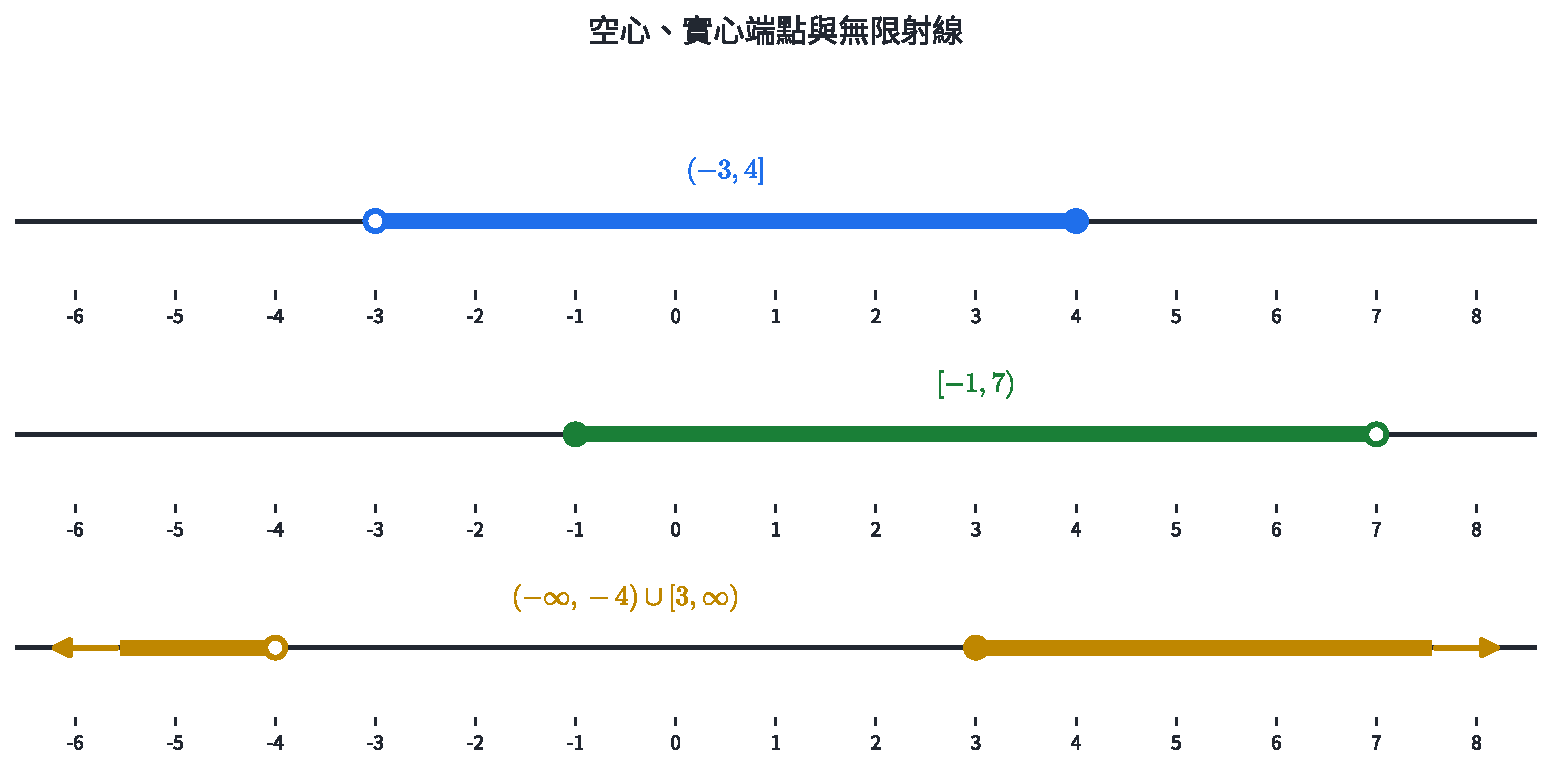
\includegraphics[width=0.92\linewidth,height=\textheight,keepaspectratio,alt={圖 1｜實數、區間端點與聯集在同一條數線上的表示。}]{assets/數1-1-實數與區間.pdf}
\caption{圖 1｜實數、區間端點與聯集在同一條數線上的表示。}
\end{figure}

比較含根式的正數時，可先確認兩邊非負，再平方。平方在非負實數上保序：若 \(a,b\ge0\)，則 \(a<b\iff a^2<b^2\)。

\subsection{例 3｜比較兩個根式和}\label{ux4f8b-3ux6bd4ux8f03ux5169ux500bux6839ux5f0fux548c}

比較 \(\sqrt{11}+\sqrt2\) 與 \(\sqrt8+\sqrt5\)。

兩者皆正，平方後比較：

\[
(\sqrt{11}+\sqrt2)^2=13+2\sqrt{22},
\]

\[
(\sqrt8+\sqrt5)^2=13+2\sqrt{40}.
\]

因 \(22<40\)，所以 \(\sqrt{22}<\sqrt{40}\)，故

\[
\boxed{\sqrt{11}+\sqrt2<\sqrt8+\sqrt5}.
\]

\subsection{例 4｜聯集與交集}\label{ux4f8b-4ux806fux96c6ux8207ux4ea4ux96c6}

設 \(A=(-3,4]\)、\(B=[1,7)\)，求 \(A\cap B\) 與 \(A\cup B\)。

共同部分從 \(1\) 到 \(4\)，兩端都包含，故 \(A\cap B=[1,4]\)。兩區間彼此重疊，合併後從 \(-3\) 延伸到 \(7\)，兩端都不含，故 \(A\cup B=(-3,7)\)。

\subsubsection{練習 1B}\label{ux7df4ux7fd2-1b}

\begin{enumerate}
\def\labelenumi{\arabic{enumi}.}
\tightlist
\item
  把 \(-2<x\le5\) 寫成區間。
\item
  設 \(A=(-\infty,2)\)、\(B=[-1,4]\)，求 \(A\cap B\) 與 \(A\cup B\)。
\item
  比較 \(3+\sqrt7\) 與 \(2\sqrt6\)。
\item
  解聯立條件 \(x>-4\) 且 \(x\le1\)，用區間表示。
\item
  一感測器的合格範圍為 \([9.95,10.05]\) V。讀值 \(9.94,9.98,10.05,10.06\) 中哪些合格？
\end{enumerate}

\section{2. 分點公式、距離與絕對值}\label{ux5206ux9edeux516cux5f0fux8dddux96e2ux8207ux7d55ux5c0dux503c}

\subsection{2.1 內分點與外分點}\label{ux5167ux5206ux9edeux8207ux5916ux5206ux9ede}

數線上 \(A(a)\)、\(B(b)\) 兩點的距離為 \(|b-a|\)。若 \(P(x)\) 位於兩點之間，且

\[
AP:PB=m:n\qquad(m,n>0),
\]

則 \(P\) 把從 \(a\) 到 \(b\) 的總位移分成 \(m:n\)。由

\[
\frac{x-a}{b-x}=\frac mn
\]

可得

\[
\boxed{x=\frac{na+mb}{m+n}}.
\]

公式中靠近 \(a\) 的權重是 \(n\)，靠近 \(b\) 的權重是 \(m\)；當 \(m=n=1\) 時得到中點 \((a+b)/2\)。

若分點在 \(AB\) 外側，圖形的先後次序會改變。依實際位置寫距離，再解比例，可同時判斷外分點在左側或右側。

\begin{figure}
\centering
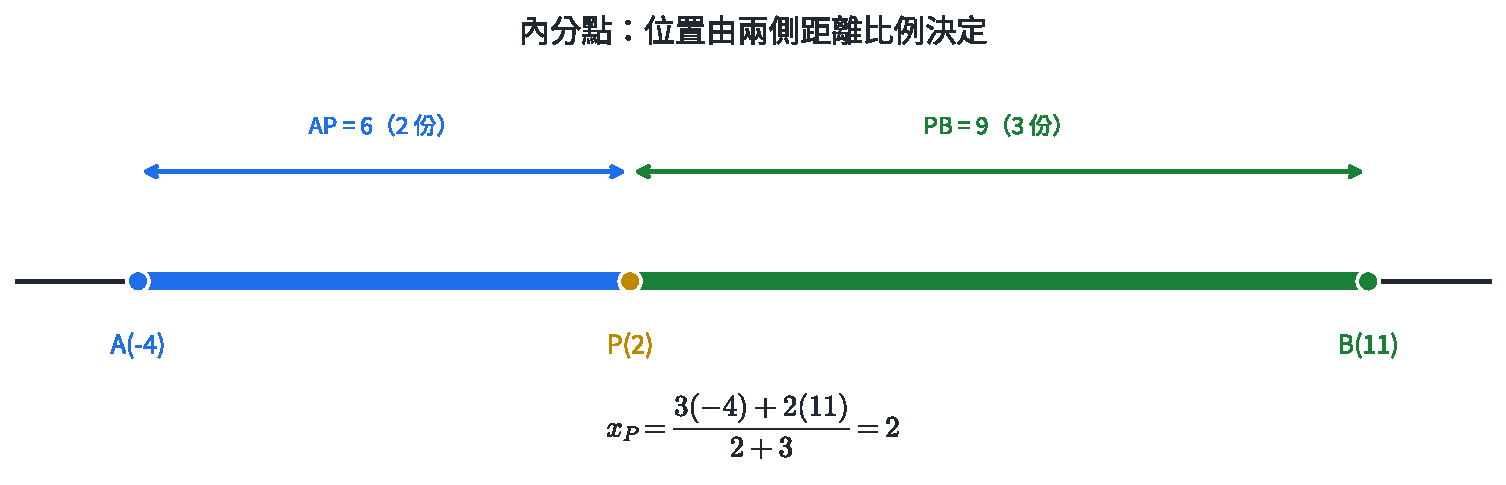
\includegraphics[width=0.9\linewidth,height=\textheight,keepaspectratio,alt={圖 2｜內分點公式來自兩段距離之比；權重與對側線段長度相配。}]{assets/數1-1-分點與距離.pdf}
\caption{圖 2｜內分點公式來自兩段距離之比；權重與對側線段長度相配。}
\end{figure}

\subsection{例 5｜內分點坐標}\label{ux4f8b-5ux5167ux5206ux9edeux5750ux6a19}

\(A(-4)\)、\(B(11)\)，點 \(P\) 在 \(AB\) 之間且 \(AP:PB=2:3\)。求 \(P\)。

\[
x_P=\frac{3(-4)+2(11)}{2+3}=\frac{10}{5}=\boxed2.
\]

檢查：\(AP=6\)、\(PB=9\)，比例為 \(2:3\)。

\subsection{例 6｜外分點由距離列式}\label{ux4f8b-6ux5916ux5206ux9edeux7531ux8dddux96e2ux5217ux5f0f}

\(A(1)\)、\(B(7)\)，點 \(Q\) 在 \(A\) 左側且 \(QA:QB=2:5\)。求 \(Q\)。

設 \(Q(x)\) 且 \(x<1\)，則 \(QA=1-x\)、\(QB=7-x\)：

\[
\frac{1-x}{7-x}=\frac25.
\]

解得 \(5-5x=14-2x\)，所以 \(x=-3\)。檢查 \(QA=4\)、\(QB=10\)，比例確為 \(2:5\)。

\subsubsection{練習 2A}\label{ux7df4ux7fd2-2a}

\begin{enumerate}
\def\labelenumi{\arabic{enumi}.}
\tightlist
\item
  \(A(-2)\)、\(B(8)\)，\(P\) 內分 \(AB\) 且 \(AP:PB=3:2\)，求 \(P\)。
\item
  求 \(A(5)\)、\(B(-7)\) 的中點。
\item
  \(A(0)\)、\(B(12)\)，點 \(Q\) 在 \(B\) 右側且 \(QA:QB=5:2\)，求 \(Q\)。
\item
  兩個測站坐標為 \(-6\) km 與 \(14\) km，設備設在兩站之間，距左站與右站之比為 \(3:2\)。求設備坐標及兩段距離。
\end{enumerate}

\subsection{2.2 絕對值是數線距離}\label{ux7d55ux5c0dux503cux662fux6578ux7ddaux8dddux96e2}

絕對值的代數定義為

\[
|x|=\begin{cases}
x,&x\ge0,\\
-x,&x<0.
\end{cases}
\]

幾何上，\(|x|\) 是 \(x\) 到原點的距離，\(|x-a|\) 是 \(x\) 到 \(a\) 的距離。因此，當 \(r>0\)：

\[
|x-a|<r\iff a-r<x<a+r,
\]

\[
|x-a|>r\iff x<a-r\ \text{或}\ x>a+r.
\]

等號版本只需把相應端點納入。若右側半徑為 \(0\) 或負數，直接由距離非負判斷解集。

三角不等式

\[
\boxed{|u+v|\le |u|+|v|}
\]

表示先走位移 \(u\) 再走位移 \(v\)，起終點直線距離不超過總路程。由 \(u=(u-v)+v\) 可進一步得到

\[
\boxed{\bigl||u|-|v|\bigr|\le|u-v|}.
\]

\begin{figure}
\centering
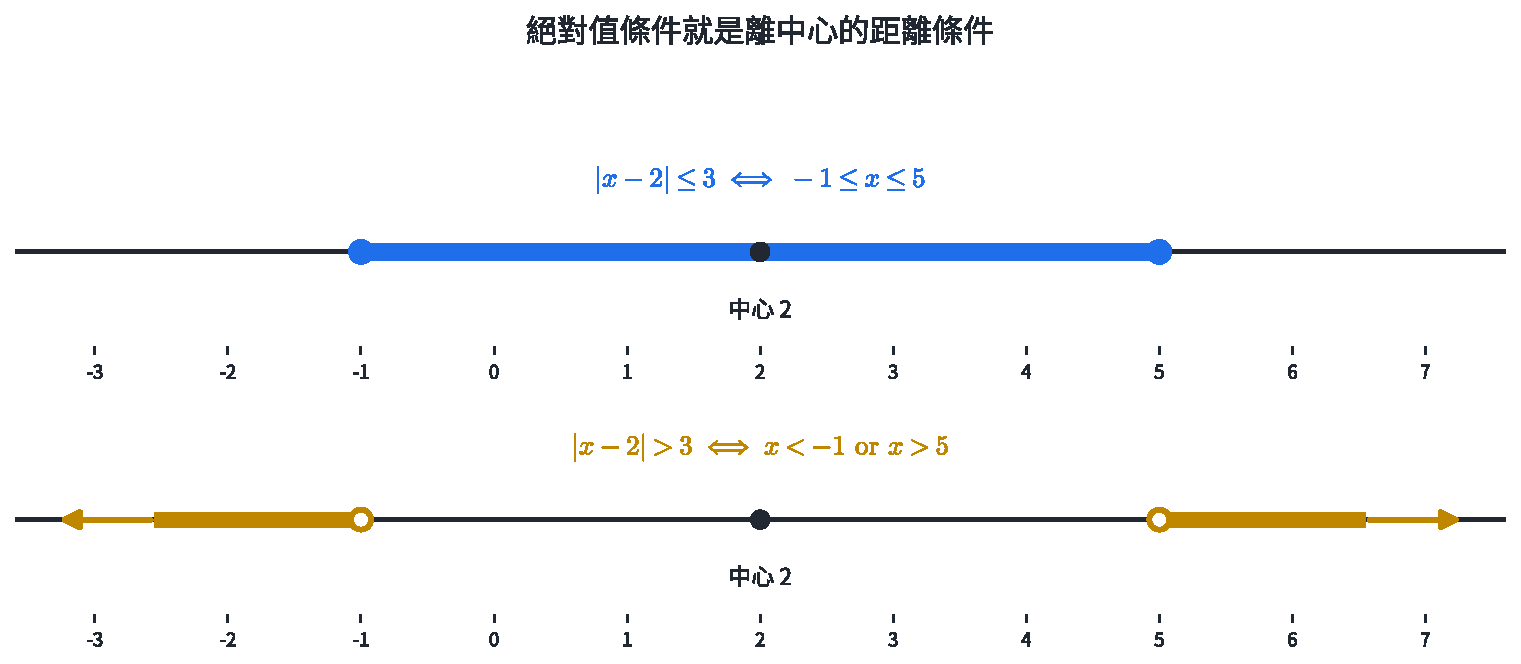
\includegraphics[width=0.92\linewidth,height=\textheight,keepaspectratio,alt={圖 3｜絕對值方程與不等式對應到固定中心的距離。}]{assets/數1-1-絕對值距離.pdf}
\caption{圖 3｜絕對值方程與不等式對應到固定中心的距離。}
\end{figure}

\subsection{例 7｜單一絕對值不等式}\label{ux4f8b-7ux55aeux4e00ux7d55ux5c0dux503cux4e0dux7b49ux5f0f}

解 \(|3x-2|\le7\)。

\[
-7\le3x-2\le7
\iff -5\le3x\le9
\iff -\frac53\le x\le3.
\]

解集為 \(\boxed{[-5/3,3]}\)。

\subsection{例 8｜兩個距離的和}\label{ux4f8b-8ux5169ux500bux8dddux96e2ux7684ux548c}

解 \(|x+1|+|x-4|\le7\)。

變號點為 \(-1,4\)。

\begin{itemize}
\tightlist
\item
  \(x<-1\)：左式 \(=-x-1+4-x=3-2x\)，得 \(x\ge-2\)，與本段交集為 \([-2,-1)\)。
\item
  \(-1\le x\le4\)：左式 \(=x+1+4-x=5\)，整段成立。
\item
  \(x>4\)：左式 \(=x+1+x-4=2x-3\)，得 \(x\le5\)，與本段交集為 \((4,5]\)。
\end{itemize}

合併得 \(\boxed{[-2,5]}\)。這也符合距離圖：在 \([-1,4]\) 內距離和固定為 \(5\)，向外每移動 \(1\)，距離和增加 \(2\)。

\subsubsection{練習 2B}\label{ux7df4ux7fd2-2b}

\begin{enumerate}
\def\labelenumi{\arabic{enumi}.}
\tightlist
\item
  解 \(|x-5|=3\)。
\item
  解 \(|2x+3|<5\)。
\item
  解 \(|x-2|\ge4\)，用區間表示。
\item
  解 \(|x+2|+|x-3|=9\)。
\item
  某零件長度 \(L\) 的目標為 \(80\) mm，容許誤差 \(0.4\) mm。分別用絕對值與區間寫出合格條件。
\item
  已知 \(|a-3|\le0.2\)、\(|b-5|\le0.1\)，利用三角不等式估計 \(|(a+b)-8|\) 的上界。
\end{enumerate}

\section{3. 乘法公式與分式}\label{ux4e58ux6cd5ux516cux5f0fux8207ux5206ux5f0f}

\subsection{3.1 公式來自分配律}\label{ux516cux5f0fux4f86ux81eaux5206ux914dux5f8b}

乘法公式是分配律的結構化結果。例如

\[
(a+b)^2=(a+b)(a+b)=a^2+2ab+b^2.
\]

常用公式包括

\[
\begin{aligned}
(a\pm b)^2&=a^2\pm2ab+b^2,\\
a^2-b^2&=(a-b)(a+b),\\
(a+b+c)^2&=a^2+b^2+c^2+2ab+2bc+2ca,\\
(a\pm b)^3&=a^3\pm3a^2b+3ab^2\pm b^3,\\
a^3+b^3&=(a+b)(a^2-ab+b^2),\\
a^3-b^3&=(a-b)(a^2+ab+b^2).
\end{aligned}
\]

展開、因式分解與代值是同一組等式的不同方向。先辨認平方差、完全平方或立方和差，常能把多步運算縮成一行。

\begin{figure}
\centering
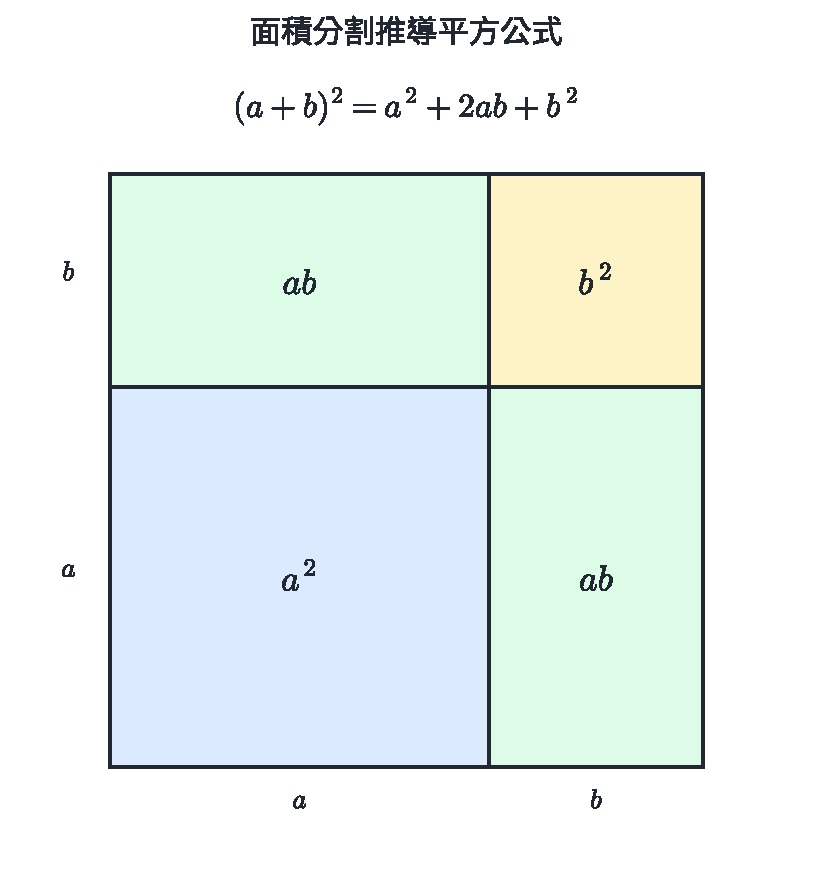
\includegraphics[width=0.82\linewidth,height=\textheight,keepaspectratio,alt={圖 4｜平方公式可由面積分割直接推得，各區塊與代數項逐一對應。}]{assets/數1-1-乘法公式面積.pdf}
\caption{圖 4｜平方公式可由面積分割直接推得，各區塊與代數項逐一對應。}
\end{figure}

\subsection{例 9｜利用結構快速計算}\label{ux4f8b-9ux5229ux7528ux7d50ux69cbux5febux901fux8a08ux7b97}

計算 \(1003^2-997^2\)。

用平方差：

\[
(1003-997)(1003+997)=6\times2000=\boxed{12000}.
\]

\subsection{例 10｜由對稱和求高次式}\label{ux4f8b-10ux7531ux5c0dux7a31ux548cux6c42ux9ad8ux6b21ux5f0f}

已知 \(x+\dfrac1x=5\)，求 \(x^2+\dfrac1{x^2}\) 與 \(x^3+\dfrac1{x^3}\)。

因 \(x\ne0\)，平方得

\[
x^2+2+\frac1{x^2}=25,
\]

所以 \(x^2+1/x^2=23\)。再用

\[
\left(x+\frac1x\right)^3=x^3+\frac1{x^3}+3\left(x+\frac1x\right),
\]

得到 \(x^3+1/x^3=125-15=\boxed{110}\)。

\subsubsection{練習 3A}\label{ux7df4ux7fd2-3a}

\begin{enumerate}
\def\labelenumi{\arabic{enumi}.}
\tightlist
\item
  展開 \((2x-3y)^3\)。
\item
  因式分解 \(8a^3-27b^3\)。
\item
  計算 \(204^2-196^2\)。
\item
  已知 \(t-1/t=4\)，求 \(t^2+1/t^2\)。
\item
  已知 \(a+b+c=10\)、\(ab+bc+ca=27\)，求 \(a^2+b^2+c^2\)。
\end{enumerate}

\subsection{3.2 分式的定義域與等值變形}\label{ux5206ux5f0fux7684ux5b9aux7fa9ux57dfux8207ux7b49ux503cux8b8aux5f62}

分式的分母必須非零。約分時消去的是共同的非零因式，因此化簡後仍要保留原式的限制。例如

\[
\frac{x^2-1}{x-1}=x+1\qquad(x\ne1).
\]

兩式在 \(x\ne1\) 時值相同；原式在 \(x=1\) 沒有定義。分式加減先分解分母並取公分母，乘除則先因式分解再約分，通常能降低展開量。

\subsection{例 11｜分式化簡並保留條件}\label{ux4f8b-11ux5206ux5f0fux5316ux7c21ux4e26ux4fddux7559ux689dux4ef6}

化簡

\[
\frac{x^2-4}{x^2-x-2}\div\frac{x+2}{x-1}.
\]

原式要求 \(x^2-x-2\ne0\)、\(x-1\ne0\)，且除式 \((x+2)/(x-1)\ne0\)，所以 \(x\ne-2,-1,1,2\)。因

\[
x^2-4=(x-2)(x+2),\qquad x^2-x-2=(x-2)(x+1),
\]

原式為

\[
\frac{(x-2)(x+2)}{(x-2)(x+1)}\cdot\frac{x-1}{x+2}
=\boxed{\frac{x-1}{x+1}},
\]

條件仍為 \(x\ne-2,-1,1,2\)。

\subsection{例 12｜通分後利用平方差}\label{ux4f8b-12ux901aux5206ux5f8cux5229ux7528ux5e73ux65b9ux5dee}

化簡 \(\dfrac1{x-3}-\dfrac1{x+3}\)。

當 \(x\ne\pm3\)：

\[
\frac{x+3-(x-3)}{(x-3)(x+3)}
=\boxed{\frac6{x^2-9}}.
\]

\subsubsection{練習 3B}\label{ux7df4ux7fd2-3b}

\begin{enumerate}
\def\labelenumi{\arabic{enumi}.}
\tightlist
\item
  化簡 \(\dfrac{x^2-9}{x^2+5x+6}\)，並寫出原式限制。
\item
  化簡 \(\dfrac2{x-1}+\dfrac3{x+1}\)。
\item
  化簡 \(\dfrac{x^2-1}{x^2-2x+1}\cdot\dfrac{x-1}{x+1}\)，並寫出限制。
\item
  解方程 \(\dfrac1{x-2}+\dfrac1{x+2}=\dfrac12\)，並檢查定義域。
\end{enumerate}

\section{4. 根式與有理化}\label{ux6839ux5f0fux8207ux6709ux7406ux5316}

對 \(a\ge0\)，\(\sqrt a\) 表示平方後等於 \(a\) 的非負實數。因此

\[
\boxed{\sqrt{x^2}=|x|}.
\]

當 \(a,b\ge0\) 時，\(\sqrt{ab}=\sqrt a\sqrt b\)；當 \(a\ge0,b>0\) 時，\(\sqrt{a/b}=\sqrt a/\sqrt b\)。這些條件保證根號都在實數範圍內。

分母有根式時，可乘以適當因式使分母成為有理數。若分母為 \(a+\sqrt b\)，常乘以共軛式 \(a-\sqrt b\)，利用

\[
(a+\sqrt b)(a-\sqrt b)=a^2-b.
\]

雙重根式可由平方公式反推。若

\[
\sqrt{A+2\sqrt B}=\sqrt m+\sqrt n,
\]

則必須有 \(m+n=A\)、\(mn=B\) 且 \(m,n\ge0\)。

\subsection{例 13｜共軛式有理化}\label{ux4f8b-13ux5171ux8edbux5f0fux6709ux7406ux5316}

化簡 \(\dfrac4{3-\sqrt5}\)。

\[
\frac4{3-\sqrt5}\cdot\frac{3+\sqrt5}{3+\sqrt5}
=\frac{4(3+\sqrt5)}{9-5}
=\boxed{3+\sqrt5}.
\]

\subsection{例 14｜化簡雙重根式}\label{ux4f8b-14ux5316ux7c21ux96d9ux91cdux6839ux5f0f}

化簡 \(\sqrt{11-6\sqrt2}\)。

尋找 \(m+n=11\)、\(mn=18\)，可取 \(m=9,n=2\)。因

\[
(3-\sqrt2)^2=11-6\sqrt2
\]

且 \(3-\sqrt2>0\)，所以

\[
\sqrt{11-6\sqrt2}=\boxed{3-\sqrt2}.
\]

\subsubsection{練習 4A}\label{ux7df4ux7fd2-4a}

\begin{enumerate}
\def\labelenumi{\arabic{enumi}.}
\tightlist
\item
  化簡 \(\sqrt{72}-2\sqrt8+\sqrt{18}\)。
\item
  化簡 \(\sqrt{(x-4)^2}\)。
\item
  有理化 \(\dfrac5{\sqrt7}\)。
\item
  有理化 \(\dfrac2{\sqrt6+\sqrt2}\)。
\item
  化簡 \(\sqrt{13+4\sqrt{10}}\)。
\end{enumerate}

\section{5. 算幾不等式與最佳值}\label{ux7b97ux5e7eux4e0dux7b49ux5f0fux8207ux6700ux4f73ux503c}

對 \(a,b\ge0\)，因平方恆非負：

\[
(\sqrt a-\sqrt b)^2\ge0.
\]

展開並整理：

\[
a+b-2\sqrt{ab}\ge0
\iff
\boxed{\frac{a+b}{2}\ge\sqrt{ab}}.
\]

左側是算術平均數，右側是幾何平均數；等號成立恰在 \(a=b\)。若 \(a,b>0\)，把 \(b\) 換成 \(k/x\) 可得

\[
x+\frac{k}{x}\ge2\sqrt k\qquad(x>0,k>0),
\]

等號在 \(x=\sqrt k\) 成立。最佳值題要同時交代「界線」與「能否取到等號」。

\begin{figure}
\centering
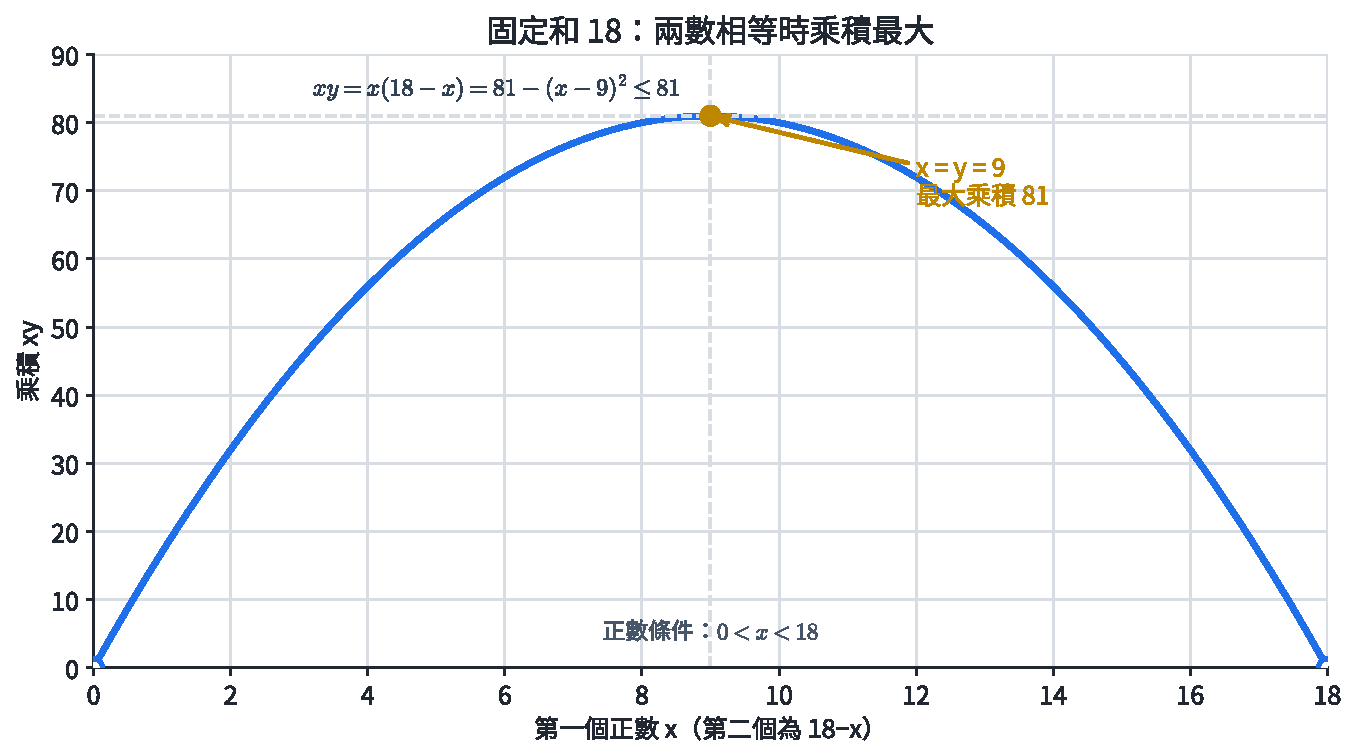
\includegraphics[width=0.86\linewidth,height=\textheight,keepaspectratio,alt={圖 5｜固定和時兩數越接近，乘積越大；相等處達到算幾不等式的等號。}]{assets/數1-1-算幾最佳化.pdf}
\caption{圖 5｜固定和時兩數越接近，乘積越大；相等處達到算幾不等式的等號。}
\end{figure}

\subsection{例 15｜固定和求最大乘積}\label{ux4f8b-15ux56faux5b9aux548cux6c42ux6700ux5927ux4e58ux7a4d}

正數 \(x,y\) 滿足 \(x+y=18\)，求 \(xy\) 的最大值。

\[
\frac{x+y}{2}\ge\sqrt{xy}
\Rightarrow 9\ge\sqrt{xy}
\Rightarrow xy\le81.
\]

當 \(x=y=9\) 時等號成立，所以最大值為 \(\boxed{81}\)。

\subsection{例 16｜固定面積求最短周長}\label{ux4f8b-16ux56faux5b9aux9762ux7a4dux6c42ux6700ux77edux5468ux9577}

矩形長寬 \(x,y>0\) 且面積 \(xy=48\)。求最小周長。

\[
x+y\ge2\sqrt{xy}=2\sqrt{48}=8\sqrt3.
\]

周長 \(P=2(x+y)\ge16\sqrt3\)。等號在 \(x=y=\sqrt{48}=4\sqrt3\) 成立，因此最小周長為 \(\boxed{16\sqrt3}\)。

\subsubsection{練習 5A}\label{ux7df4ux7fd2-5a}

\begin{enumerate}
\def\labelenumi{\arabic{enumi}.}
\tightlist
\item
  正數 \(a,b\) 滿足 \(a+b=30\)，求 \(ab\) 最大值與等號條件。
\item
  對 \(x>0\)，求 \(x+16/x\) 的最小值。
\item
  對 \(x>2\)，求 \((x-2)+9/(x-2)\) 的最小值。
\item
  面積為 \(100\text{ m}^2\) 的長方形花圃，求最短周長及長寬。
\item
  正數 \(p,q\) 滿足 \(pq=12\)，求 \(3p+4q\) 的最小值。
\end{enumerate}

\section{6. 分節練習完整解析}\label{ux5206ux7bc0ux7df4ux7fd2ux5b8cux6574ux89e3ux6790}

\subsection{練習 1A}\label{ux7df4ux7fd2-1a-1}

\begin{enumerate}
\def\labelenumi{\arabic{enumi}.}
\tightlist
\item
  設 \(x=0.\overline{54}\)，則 \(100x-x=54\)，故 \(x=54/99=\boxed{6/11}\)。
\item
  設 \(x=2.3\overline{18}\)，則 \(10x=23.\overline{18}\)、\(1000x=2318.\overline{18}\)。相減得 \(990x=2295\)，故 \(x=\boxed{51/22}\)。
\item
  \(8^2=64<70<81=9^2\)，故 \(\boxed{8<\sqrt{70}<9}\)。
\item
  \(\sqrt{18}-3\sqrt2=3\sqrt2-3\sqrt2=0\)，是有理數；\(0.1010010001\ldots\) 不終止且不循環，是無理數；\(-7/4\) 是有理數。
\item
  假設 \(r+u=s\) 是有理數，則 \(u=s-r\) 為兩個有理數之差，也會是有理數，與已知矛盾。因此 \(r+u\) 是無理數。
\item
  \(40=2^3\cdot5\)，故 \(7/40\) 為有限小數；\(24=2^3\cdot3\) 含質因數 \(3\)，故最簡分數 \(11/24\) 為循環小數。
\end{enumerate}

\subsection{練習 1B}\label{ux7df4ux7fd2-1b-1}

\begin{enumerate}
\def\labelenumi{\arabic{enumi}.}
\tightlist
\item
  \(\boxed{(-2,5]}\)。
\item
  \(A\cap B=\boxed{[-1,2)}\)；\(A\cup B=\boxed{(-\infty,4]}\)。
\item
  兩數皆正。\((3+\sqrt7)^2=16+6\sqrt7>24=(2\sqrt6)^2\)，故 \(\boxed{3+\sqrt7>2\sqrt6}\)。
\item
  同時滿足兩條件得 \(\boxed{(-4,1]}\)。
\item
  合格讀值為 \(\boxed{9.98,10.05}\) V；端點 \(10.05\) 包含在閉區間內。
\end{enumerate}

\subsection{練習 2A}\label{ux7df4ux7fd2-2a-1}

\begin{enumerate}
\def\labelenumi{\arabic{enumi}.}
\tightlist
\item
  \(x_P=[2(-2)+3(8)]/5=\boxed4\)。
\item
  中點為 \((5-7)/2=\boxed{-1}\)。
\item
  設 \(Q(x)\) 且 \(x>12\)，則 \(x:(x-12)=5:2\)，解得 \(x=\boxed{20}\)。
\item
  坐標為 \([2(-6)+3(14)]/5=\boxed6\) km；距離為 \(12\) km 與 \(8\) km，比例 \(3:2\)。
\end{enumerate}

\subsection{練習 2B}\label{ux7df4ux7fd2-2b-1}

\begin{enumerate}
\def\labelenumi{\arabic{enumi}.}
\tightlist
\item
  \(x-5=\pm3\)，故 \(\boxed{x=2,8}\)。
\item
  \(-5<2x+3<5\)，得 \(-8<2x<2\)，所以 \(\boxed{-4<x<1}\)。
\item
  \(x-2\le-4\) 或 \(x-2\ge4\)，故 \(\boxed{(-\infty,-2]\cup[6,\infty)}\)。
\item
  變號點為 \(-2,3\)。中段距離和為 \(5\)；左段解得 \(x=-4\)，右段解得 \(x=5\)，故 \(\boxed{x=-4,5}\)。
\item
  \(\boxed{|L-80|\le0.4}\)，等價區間為 \(\boxed{[79.6,80.4]}\) mm。
\item
  \(|(a+b)-8|=|(a-3)+(b-5)|\le|a-3|+|b-5|\le\boxed{0.3}\)。
\end{enumerate}

\subsection{練習 3A}\label{ux7df4ux7fd2-3a-1}

\begin{enumerate}
\def\labelenumi{\arabic{enumi}.}
\tightlist
\item
  \((2x-3y)^3=\boxed{8x^3-36x^2y+54xy^2-27y^3}\)。
\item
  \(8a^3-27b^3=\boxed{(2a-3b)(4a^2+6ab+9b^2)}\)。
\item
  \((204-196)(204+196)=8\times400=\boxed{3200}\)。
\item
  \((t-1/t)^2=t^2-2+1/t^2=16\)，故 \(t^2+1/t^2=\boxed{18}\)。
\item
  \((a+b+c)^2=a^2+b^2+c^2+2(ab+bc+ca)\)，故所求 \(=100-54=\boxed{46}\)。
\end{enumerate}

\subsection{練習 3B}\label{ux7df4ux7fd2-3b-1}

\begin{enumerate}
\def\labelenumi{\arabic{enumi}.}
\tightlist
\item
  \(\dfrac{(x-3)(x+3)}{(x+2)(x+3)}=\boxed{\dfrac{x-3}{x+2}}\)，原式限制 \(\boxed{x\ne-3,-2}\)。
\item
  公分母為 \(x^2-1\)，結果為 \(\boxed{\dfrac{5x-1}{x^2-1}}\)，\(x\ne\pm1\)。
\item
  化簡為 \(\boxed1\)，原式限制 \(\boxed{x\ne1,-1}\)。
\item
  定義域要求 \(x\ne\pm2\)。通分得 \(2x/(x^2-4)=1/2\)，即 \(x^2-4x-4=0\)，故 \(\boxed{x=2\pm2\sqrt2}\)，兩解都在定義域內。
\end{enumerate}

\subsection{練習 4A}\label{ux7df4ux7fd2-4a-1}

\begin{enumerate}
\def\labelenumi{\arabic{enumi}.}
\tightlist
\item
  \(6\sqrt2-4\sqrt2+3\sqrt2=\boxed{5\sqrt2}\)。
\item
  \(\boxed{|x-4|}\)。
\item
  \(\dfrac5{\sqrt7}=\boxed{\dfrac{5\sqrt7}{7}}\)。
\item
  乘以共軛式後得 \(2(\sqrt6-\sqrt2)/(6-2)=\boxed{(\sqrt6-\sqrt2)/2}\)。
\item
  取 \(m+n=13,mn=40\)，得 \(m=8,n=5\)，所以 \(\boxed{2\sqrt2+\sqrt5}\)。
\end{enumerate}

\subsection{練習 5A}\label{ux7df4ux7fd2-5a-1}

\begin{enumerate}
\def\labelenumi{\arabic{enumi}.}
\tightlist
\item
  \(ab\le[(a+b)/2]^2=225\)，最大值 \(\boxed{225}\)，在 \(a=b=15\) 成立。
\item
  \(x+16/x\ge2\sqrt{16}=\boxed8\)，在 \(x=4\) 成立。
\item
  令 \(u=x-2>0\)，則 \(u+9/u\ge\boxed6\)，在 \(u=3\)、即 \(x=5\) 成立。
\item
  長寬相等時周長最短，故長寬皆為 \(10\) m，最短周長 \(\boxed{40\text{ m}}\)。
\item
  \(3p+4q=3p+48/p\ge2\sqrt{144}=\boxed{24}\)，等號在 \(3p=48/p\)，得 \(p=4,q=3\)。
\end{enumerate}

\section{7. 章末代表題}\label{ux7ae0ux672bux4ee3ux8868ux984c}

\subsection{基礎與核心}\label{ux57faux790eux8207ux6838ux5fc3}

\begin{enumerate}
\def\labelenumi{\arabic{enumi}.}
\tightlist
\item
  將 \(0.2\overline{7}\) 化成最簡分數。
\item
  求滿足 \(3\le\sqrt n<4\) 的正整數 \(n\)。
\item
  設 \(A=(-5,2]\)、\(B=[-1,6)\)，求 \(A\cap B\) 與 \(A\cup B\)。
\item
  \(A(-8)\)、\(B(7)\)，點 \(P\) 內分 \(AB\) 且 \(AP:PB=4:1\)，求 \(P\)。
\item
  解 \(|2x-5|\le9\)。
\item
  解 \(|x-1|+|x+3|>8\)。
\item
  因式分解 \(x^6-64\)。
\item
  化簡 \(\dfrac{x^2-4x+4}{x^2-4}\)，並寫出原式限制。
\end{enumerate}

\subsection{進階}\label{ux9032ux968e}

\begin{enumerate}
\def\labelenumi{\arabic{enumi}.}
\setcounter{enumi}{8}
\tightlist
\item
  化簡 \(\sqrt{48}+\sqrt{27}-\sqrt{75}\)。
\item
  化簡 \(\dfrac1{\sqrt5-2}-\dfrac1{\sqrt5+2}\)。
\item
  已知 \(a+1/a=3\)，求 \(a^4+1/a^4\)。
\item
  對 \(x>0\)，求 \(2x+18/x\) 的最小值及等號條件。
\end{enumerate}

\subsection{跨節整合}\label{ux8de8ux7bc0ux6574ux5408}

\begin{enumerate}
\def\labelenumi{\arabic{enumi}.}
\setcounter{enumi}{12}
\tightlist
\item
  某製程的合格濃度為 \(|c-12|\le0.3\)。兩次獨立校正可能分別造成不超過 \(0.08\) 與 \(0.05\) 的加法偏移。若儀器顯示 \(12.20\)，用三角不等式給出真值相對 \(12\) 的最大可能偏差，並判斷能否保證合格。
\item
  數線上 \(A(-2)\)、\(B(10)\)，\(P\) 內分 \(AB\) 且 \(AP:PB=1:2\)。求 \(P\)，再解 \(|x-P|\le AP/2\)。
\item
  一長方形展示板面積固定為 \(72\text{ dm}^2\)。邊框每公尺材料價格相同，求使邊框成本最低的長寬與周長；答案保留根式。
\item
  設 \(u=\sqrt5+2\)。先有理化求 \(1/u\)，再求 \(u^2+1/u^2\)，最後比較此值與 \(18\)。
\end{enumerate}

\section{8. 章末代表題完整詳解}\label{ux7ae0ux672bux4ee3ux8868ux984cux5b8cux6574ux8a73ux89e3}

\begin{enumerate}
\def\labelenumi{\arabic{enumi}.}
\item
  設 \(x=0.2\overline7\)。則 \(10x=2.\overline7\)、\(100x=27.\overline7\)，相減得 \(90x=25\)，所以 \(\boxed{x=5/18}\)。
\item
  平方在非負數上保序：\(9\le n<16\)。正整數為 \(\boxed{9,10,11,12,13,14,15}\)。
\item
  共同部分為 \(\boxed{[-1,2]}\)；合併範圍為 \(\boxed{(-5,6)}\)。
\item
  \(x_P=[1(-8)+4(7)]/5=20/5=\boxed4\)。檢查 \(AP=12,PB=3\)，比例為 \(4:1\)。
\item
  \(-9\le2x-5\le9\)，所以 \(-4\le2x\le14\)，解為 \(\boxed{[-2,7]}\)。
\item
  變號點為 \(-3,1\)。在中段 \([-3,1]\)，距離和固定為 \(4\)；左段左式 \(=-2x-2>8\)，得 \(x<-5\)；右段左式 \(=2x+2>8\)，得 \(x>3\)。故解集為 \(\boxed{(-\infty,-5)\cup(3,\infty)}\)。
\item
  先作平方差，再作立方和差：
\end{enumerate}

\[
x^6-64=(x^3-8)(x^3+8)
=(x-2)(x^2+2x+4)(x+2)(x^2-2x+4).
\]

\begin{enumerate}
\def\labelenumi{\arabic{enumi}.}
\setcounter{enumi}{7}
\tightlist
\item
  原式分母 \((x-2)(x+2)\)，故 \(x\ne\pm2\)。化簡得
\end{enumerate}

\[
\frac{(x-2)^2}{(x-2)(x+2)}=\boxed{\frac{x-2}{x+2}},
\]

且仍保留 \(\boxed{x\ne\pm2}\)。

\begin{enumerate}
\def\labelenumi{\arabic{enumi}.}
\setcounter{enumi}{8}
\item
  \(\sqrt{48}=4\sqrt3\)、\(\sqrt{27}=3\sqrt3\)、\(\sqrt{75}=5\sqrt3\)，所以結果為 \(\boxed{2\sqrt3}\)。
\item
  各分母互為共軛：
\end{enumerate}

\[
\frac1{\sqrt5-2}=\sqrt5+2,
\qquad
\frac1{\sqrt5+2}=\sqrt5-2.
\]

相減得 \(\boxed4\)。

\begin{enumerate}
\def\labelenumi{\arabic{enumi}.}
\setcounter{enumi}{10}
\tightlist
\item
  先平方：\(a^2+1/a^2=3^2-2=7\)。再平方：
\end{enumerate}

\[
a^4+\frac1{a^4}=7^2-2=\boxed{47}.
\]

\begin{enumerate}
\def\labelenumi{\arabic{enumi}.}
\setcounter{enumi}{11}
\item
  \(2x+18/x\ge2\sqrt{36}=12\)。等號要求 \(2x=18/x\)，故 \(x=3\)。最小值為 \(\boxed{12}\)。
\item
  儀器顯示值距目標為 \(|12.20-12|=0.20\)。兩校正偏移合計的絕對值至多 \(0.08+0.05=0.13\)，所以真值相對目標的偏差至多
\end{enumerate}

\[
0.20+0.13=\boxed{0.33}.
\]

合格門檻是 \(0.30\)，因此現有資料無法保證合格；這是上界判斷，實際偏移若互相抵銷，真值仍可能合格。

\begin{enumerate}
\def\labelenumi{\arabic{enumi}.}
\setcounter{enumi}{13}
\item
  \(P=[2(-2)+1(10)]/3=2\)。\(AP=4\)，所以 \(AP/2=2\)。條件為 \(|x-2|\le2\)，解得 \(\boxed{x\in[0,4]}\)。
\item
  設長寬 \(x,y>0\)，\(xy=72\)。周長
\end{enumerate}

\[
2(x+y)\ge4\sqrt{xy}=4\sqrt{72}=24\sqrt2.
\]

等號在 \(x=y=\sqrt{72}=6\sqrt2\) 成立。因此長、寬皆為 \(\boxed{6\sqrt2\text{ dm}}\)，最短周長為 \(\boxed{24\sqrt2\text{ dm}}\)。

\begin{enumerate}
\def\labelenumi{\arabic{enumi}.}
\setcounter{enumi}{15}
\tightlist
\item
  因 \((\sqrt5+2)(\sqrt5-2)=1\)，所以 \(1/u=\sqrt5-2\)。因此
\end{enumerate}

\[
u+\frac1u=2\sqrt5,
\]

\[
u^2+\frac1{u^2}=\left(2\sqrt5\right)^2-2=\boxed{18}.
\]

故此值與 \(18\) 相等。

\section{9. 核心整理}\label{ux6838ux5fc3ux6574ux7406}

\begin{itemize}
\tightlist
\item
  有理數可寫成整數比，小數展開有限或循環；無理數的小數展開不終止且不循環。
\item
  區間括號記錄端點是否包含；聯集對應「或」，交集對應「且」。
\item
  內分點 \(AP:PB=m:n\) 的坐標為 \((na+mb)/(m+n)\)；由距離比例推導可檢查權重位置。
\item
  \(|x-a|\) 是 \(x\) 與 \(a\) 的距離；多個絕對值以變號點切段，每段解再與該段範圍取交集。
\item
  乘法公式來自分配律。分式化簡保留原分母非零與除式非零的限制。
\item
  \(\sqrt{x^2}=|x|\)；共軛式把根式分母轉成平方差。
\item
  算幾不等式適用於非負數，等號條件決定最佳值是否可達。
\end{itemize}


\end{document}
